% !TeX spellcheck=en_GB
\section{Benchmarks}
\subsection{Benchmark Environment}
To compare to our solution with an off the shelf algorithm, the CPLEX framework was chosen, which is developed and maintained by IBM\footnote{\url{http://www-01.ibm.com/software/commerce/optimization/cplex-optimizer/index.html}}. It is available to use for students and faculty for free and is one of the most used optimization frameworks and can solve both linear and integer linear programs very efficiently.

We tested the GPU implementations on a CentOS 7 Server with an Intel E5-4660 V4 processor, 126 gb memory and with a Nvidia GTX 780ti. Both the CPLEX framework and the sequentiel 
implementation were tested on a Ubuntu 14.04 machine with 8 gb memory and an Intel i5-4200U, due to the fact that we did not have the permissions to install CPLEX on the server.

To run all the test categories, all the instance sizes with all the implementations, download \todo{download} and then run \todo{command}. This requires that you run on a machine with an available GPU and that Futhark and Python are installed.

We have chosen to benchmark on four categories of tests which represents instances where different dimensions are the dominant or limited. By doing so different weaknesses in the implementations can be revealed. First category is one instance where the dimensions of the linear program is large. Second category is many small instances to showcase how well the algorithm handles parallelism across instances. Third category contains many instances of big size to allow for huge parallelism and the fourth category contains many instances of varying size to simulate potential real data which might not always be uniform.

\subsection{One big instance}
\begin{table}[H]
	\centering
	\label{table:one-big-instance}
	\begin{tabular}{|l|l|l|l|l|l|}\hline
		Instance & cplex & seq reduced & reduced & reduced-flat & reduced-flat-multi \\\hline
		&       &             &         &              &                    \\\hline
		&       &             &         &              &                    \\\hline
		&       &             &         &              &                   \\\hline
		&       &             &         &              &                   \\\hline
		&       &             &         &              &                   \\\hline
	\end{tabular}
	\caption{My caption}
\end{table}

\begin{figure}[H]
	\centering
	\label{fig-vary}
	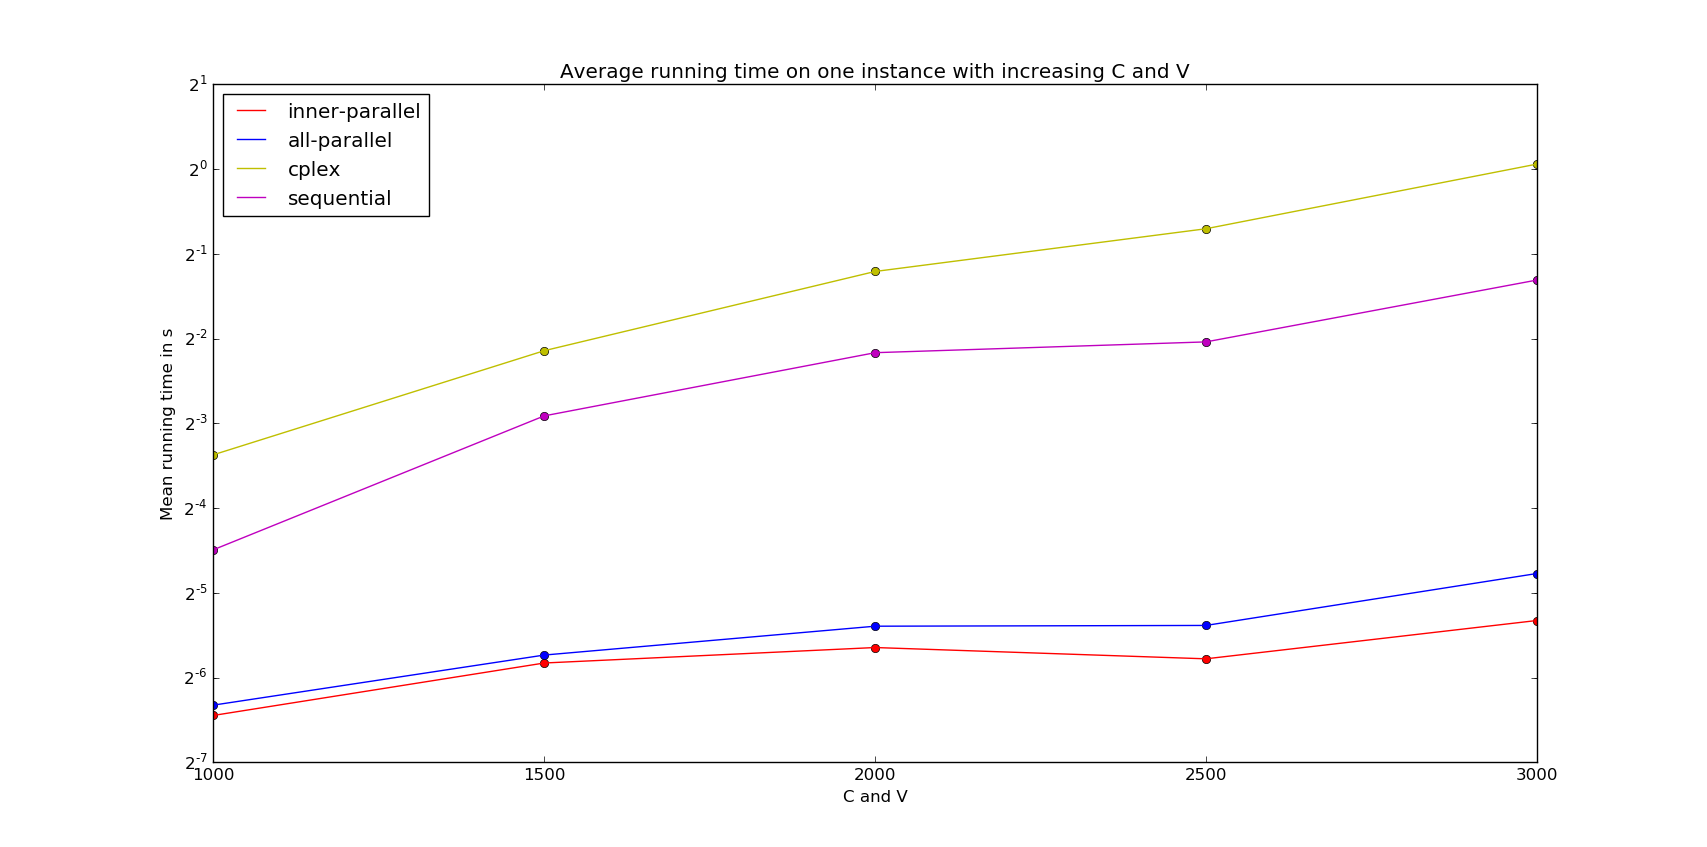
\includegraphics[width=\textwidth]{one-big}
	\caption{The average running time of the different implementations, with one instance with highnumber of C and V}
	\graphicspath{dir-list}
\end{figure}
\todo[inline]{Skal opdaters}

As seen table \ref{table:one-big-instance} the reduced-flat is the fastest implementation across all sizes. This is expected since it is fully parallel on each instance while not having as much overhead as the reduced-flat-multi. Slowest of the GPU-parallel versions is the reduced which on a single instance is sequential which is also why we see faster running times of the CPU versions that this one, hence it is only running at the clock speed of the GPU which is significantly slower than the CPU. We also see that while the CPLEX is multi threaded the Futhark C-code is competitive.

\subsection{Many small instances}
\begin{table}[H]
	\centering
	\label{table:many_small_instances}
	\begin{tabular}{|l|l|l|l|l|l|}\hline
		Instance & cplex & seq reduced & reduced & reduced-flat & reduced-flat-multi \\\hline
		&       &             &         &              &                    \\\hline
		&       &             &         &              &                    \\\hline
		&       &             &         &              &                   \\\hline
		&       &             &         &              &                   \\\hline
		&       &             &         &              &                   \\\hline
	\end{tabular}
	\caption{My caption}
\end{table}

\begin{figure}[H]
	\centering
	\label{fig-small}
	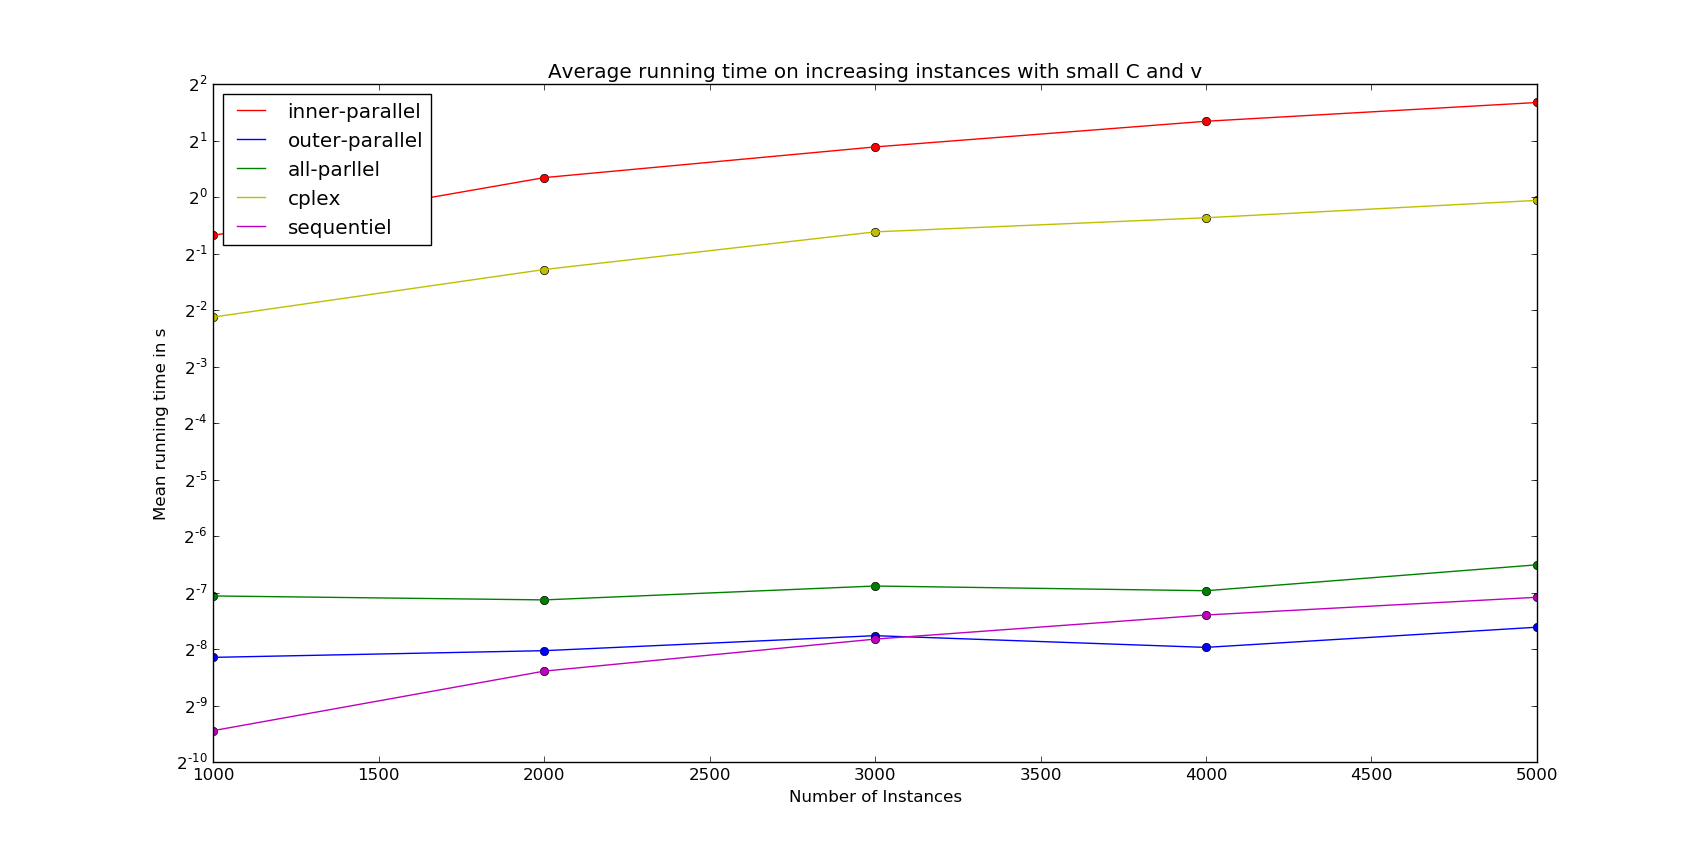
\includegraphics[width=\textwidth]{many-small}
	\caption{The average running time of the different implementations, on different sizes of N with a low number of C and V.}
	\graphicspath{dir-list}
\end{figure}
\todo[inline]{Skal opdaters}
As seen on table \ref{table:many_small_instances} the reduced version is the fastest. This is expected since it is parallel on the outer dimension which is the dominant dimension in these test cases. Since each instance only require relatively little work the reduced-flat does relatively bad. It waits for each instance to complete before the next starts which also implies that it will transfer the data over to the GPU in multiple stages, increasing the overhead of the algorithm. The reduced-flat-multi does fairly well since it is also parallel in the outer dimension but it is clear that the overhead for flattening the nested parallelism makes it slower than the reduced version. Furthermore it is clear that for a large number of instances the GPU clearly does better than the both of the CPU versions.


\subsection{Many big instances}
\begin{table}[H]
	\centering
	\label{table:many_big_instances}
	\begin{tabular}{|l|l|l|l|l|l|}\hline
		Instance & cplex & seq reduced & reduced & reduced-flat & reduced-flat-multi \\\hline
		&       &             &         &              &                    \\\hline
		&       &             &         &              &                    \\\hline
		&       &             &         &              &                   \\\hline
		&       &             &         &              &                   \\\hline
		&       &             &         &              &                   \\\hline
	\end{tabular}
	\caption{My caption}
\end{table}

\begin{figure}[H]
	\centering
	\label{fig-big}
	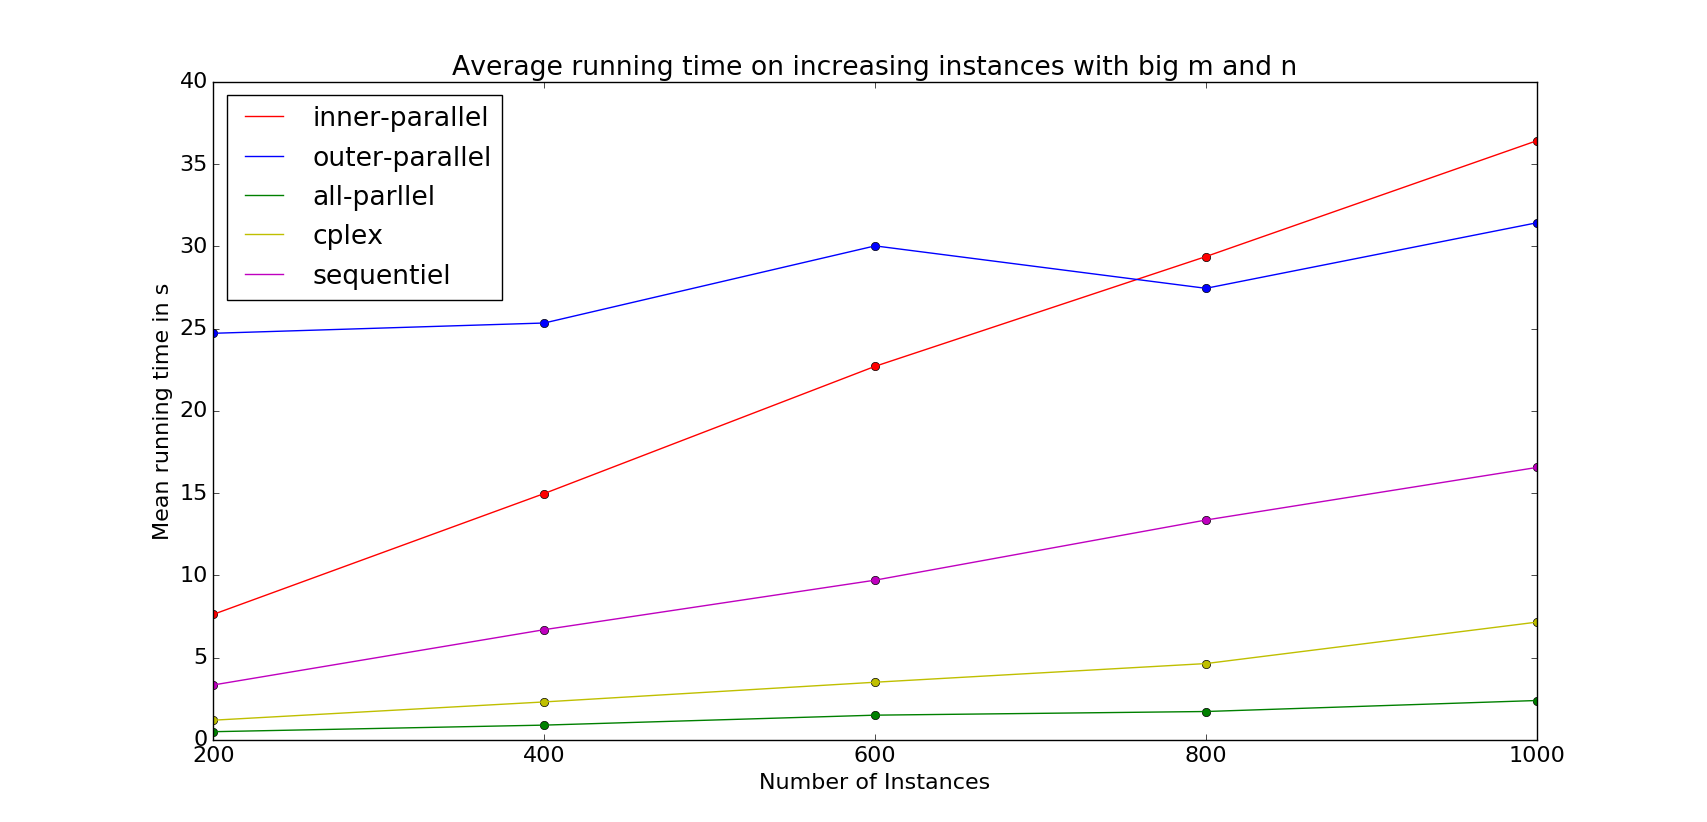
\includegraphics[width=\textwidth]{many-big}
	\caption{The average running time of the different implementations, on different sizes of N with high numbers of C and V}
	\graphicspath{dir-list}
\end{figure}
\todo[inline]{Skal opdaters}

As seen in table \ref{table:many_big_instances} the reduced-flat-multi implementation is the fastest. This was expected since it is the implementation with the highest level of parallelism on both dimensions. Since both dimensions are large it effectively utilizes the number of threads to its the fullest and the overhead of generating helper arrays becomes negligible. The reduced and reduced-flat does competitively well since both of the dimensions are big and they can utilize the parallelism which also explains wy both of these run faster than the CPU versions.

\subsection{Many instances of varying size}
\begin{table}[H]
	\centering
	\label{table:many_varying_instances}
	\begin{tabular}{|l|l|l|l|l|l|}\hline
		Instance & cplex & seq reduced & reduced & reduced-flat & reduced-flat-multi \\\hline
		&       &             &         &              &                    \\\hline
		&       &             &         &              &                    \\\hline
		&       &             &         &              &                   \\\hline
		&       &             &         &              &                   \\\hline
		&       &             &         &              &                   \\\hline
	\end{tabular}
	\caption{My caption}
\end{table}

\begin{figure}[H]
	\centering
	\label{fig-vary}
	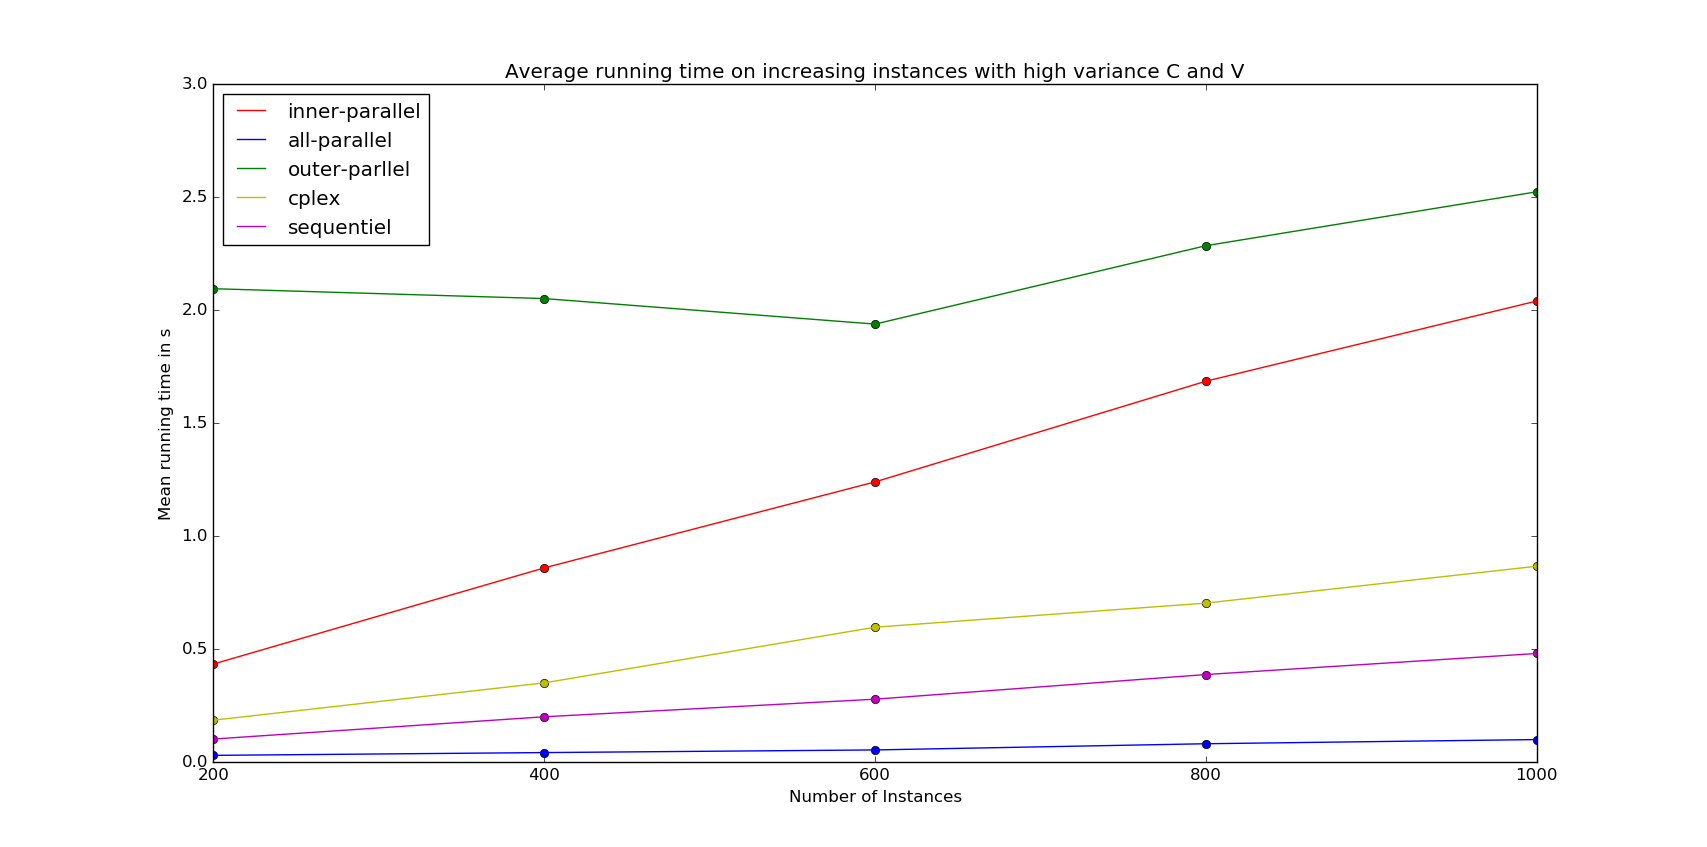
\includegraphics[width=\textwidth]{many-varying}
	\caption{The average running time of the different implementations, on different sizes of N with C and V varying a lot.}
	\graphicspath{dir-list}
\end{figure}
\todo[inline]{Skal opdaters}
As seen in table \ref{table:many_varying_instances} the reduced-flat-multi implementation shows its strength. The implementation is ambiguous on the varying sizes and utilizes this to the fullest. The weakness of the implementations which are parallel on only one dimension, is revealed when the opposite dimension is large and therefore take up time on the GPU where other threads will wait. But while reduced and reduced-flat is a factor x\todo{x} slower than the reduced-flat-multi they still achieve a factor x\todo{x} speed-up from the CPU versions.
